\documentclass[10pt,journal,letterpaper]{IEEEtran}
\usepackage[margin=1in]{geometry}
\usepackage{amsmath,amssymb,graphicx,booktabs,array,cite,url}
\usepackage[hidelinks]{hyperref}
\hypersetup{pdftitle={Classical and Self-Supervised Hankel Filtering for Magnitude-Only Rydberg Channel Estimation},pdfauthor={Abdullah Haatim}}
\graphicspath{{figures/}}
\interdisplaylinepenalty=2500
\newcommand{\CN}{\mathcal{CN}}
\newcommand{\HH}{\mathcal{H}}
\DeclareMathOperator{\diag}{diag}
\DeclareMathOperator{\tr}{tr}
\DeclareMathOperator{\sigmoid}{sigmoid}
\DeclareMathOperator{\softplus}{softplus}
\DeclareMathOperator{\median}{median}
\hyphenation{Ryd-berg mea-sure-ments}
\begin{document}
\title{Classical and Self-Supervised Hankel Filtering for Magnitude-Only Rydberg Channel Estimation}
\author{Abdullah~Haatim\thanks{A. Haatim is with the Department of Electrical and Electronics Engineering, Birla Institute of Technology and Science, Pilani, India (e-mail: f20220519@pilani.bits-pilani.ac.in).}}
\maketitle
\begin{abstract}
Rydberg atomic receivers can estimate wireless channels from signal magnitudes measured with a known reference. Spatial channel structure can remove noise, but excessive filtering can also remove useful paths. We study this trade-off through classical estimation and a compact self-supervised estimator. The learned method keeps the exact Rician measurement update and uses a small controller to adjust smooth Hankel filtering. It learns from withheld pilot measurements rather than true channels. Paired simulations show how array size, effective rank and repeated filtering affect classical recovery. A fresh comparison finds that the compact estimator improves average accuracy over global learned filtering, a residual-driven recurrent adaptation and offline-tuned OptShrink. Allowing OptShrink to choose rank separately for each received block gives better average cellwise accuracy, but requires substantially more processing in the tested implementation. The learned estimator has fewer errors above a stated severe-error threshold, without dominating the error distribution. Weak references and nearly noiseless observations remain important failures. The contribution is a measured accuracy--cost trade-off under a calibrated magnitude model, not universal superiority or a hardware demonstration.
\end{abstract}
\begin{IEEEkeywords}
Channel estimation, Hankel matrices, magnitude measurements, Rydberg receivers, self-supervised learning.
\end{IEEEkeywords}

\section{Introduction}
\IEEEPARstart{R}{ydberg} atomic receivers sense radio-frequency electric fields through highly excited atoms. Their sensitivity and broad operating range motivate research on wireless communication and sensing, including future networks~\cite{gong2025mag}. Array models extend this setting to multiple users~\cite{cui2025}. In the magnitude-only receiver considered here, a known reference combines with the incoming field before amplitude measurement. The receiver does not directly observe complex baseband samples. Recovering the complex channel is therefore a nonlinear inverse problem, even when the pilots and reference are known.

A small number of propagation paths also gives the channel structure across the array. A Hankel matrix built from a uniform linear array channel has low rank. Filtering this matrix can suppress noise, but hard truncation can erase weak paths. The appropriate amount of filtering depends on the measurements and on channel complexity. Searching for a rank separately for every received block can be expensive. This motivates a practical question: can a small learned rule reuse offline training to provide useful structural correction at lower processing cost, and when does a well-tuned classical method remain better?

This paper combines three contributions within one observation model. First, paired classical experiments relate filtering gains to array size, effective rank and the number of projection sweeps. Second, a 188-parameter estimator learns smooth spatial filtering from withheld measurements while retaining exact Rician expectation--maximization (EM) updates. Third, a fresh comparison measures its accuracy, large-error frequency and processing time against smaller learned controls and two strong OptShrink adaptations. We derive properties of individual updates and state their limits. The contribution is a compact estimation design and evidence about when it is worthwhile, not a new low-rank principle or a universally better shrinker.

\subsection{Relation to Existing Work}
Cui et al.\ developed EM-based Gerchberg--Saxton (EM-GS) for atomic-MIMO signal detection~\cite{cui2025}; our known-pilot application estimates channels. Strong-reference linearization provides another estimation approach~\cite{xu2025}; we retain exact magnitude observations. URformer unfolds phase retrieval for Rydberg receivers~\cite{xiao2026}, so neither unfolding nor the observation model is new. Our results do not reproduce its published performance. Quantum-MUSIC uses recovered channels for direction finding~\cite{kim2025quantummusic}, while a robust variant treats outliers~\cite{banerjee2026robust}. Our Gaussian-field-noise simulations do not establish that form of robustness.

Classical structure processing includes Cadzow's alternating projections~\cite{cadzow1988}, Hankel recovery~\cite{chen2014emac}, low-rank Hankel denoising (LRHD)~\cite{yin2021}, and structured alternating least squares~\cite{zachariah2012}. OptShrink chooses data-driven singular-value weights~\cite{nadakuditi2014}. Variational Bayesian low-rank phase retrieval~\cite{liu2018lrpr} and Vandermonde factorization~\cite{ying2018hvaf} offer other priors. Their original observations and guarantees differ from referenced Rician recovery. Our in-loop OptShrink adaptation is a strong control, not a reproduction of full LRHD or these other methods. Their guarantees are not transferred to the dependent errors produced by nonlinear reconstruction and Hankel lifting.

Compact learned estimators also have clear precedents. C-TISTA uses four scalars per stage for complex inverse problems~\cite{takabe2020ctista}. ALISTA retains analytic weights and learns steps and thresholds~\cite{liu2019alista}; OAMP-Net2 uses four scalars per stage for MIMO detection~\cite{he2020oamp}. NA-ALISTA uses recurrence and observed residual summaries to control sparse recovery~\cite{behrens2021naalista}. Compactness and input-dependent control are not new by themselves. Learned Hankel reconstruction~\cite{huang2021}, withheld-measurement self-supervision~\cite{yaman2020,luo2023}, Rician-likelihood learning~\cite{parker2023}, and self-supervised Rydberg-signal denoising~\cite{liu2026} also precede this work. Our specific design adjusts smooth spatial Hankel filtering inside exact referenced-magnitude EM. The matched recurrent control tests one adaptation of that broader idea, not superiority over published NA-ALISTA.

\section{System Model and Available Information}
An $N$-element array receives $P$ pilots from $K$ users:
\begin{equation}
 Z=|GS+B+W|,\qquad W_{np}\sim\CN(0,v).
 \label{eq:model}
\end{equation}
Here $G\in\mathbb C^{N\times K}$ is the unknown channel, $S\in\mathbb C^{K\times P}$ contains known pilots, and $B$ is the known reference field. Magnitude acts entrywise. Noise samples are independent, with variance $v/2$ in each real component. Receiver conversion gain is absorbed into the scaling. This effective model does not simulate atomic dynamics, optical readout or hardware drift.

For a half-wavelength uniform linear array, user $k$ has channel
\begin{equation}
 g_{nk}=\sum_{\ell=1}^{L_k}\alpha_{\ell k}e^{-j\pi n\sin\theta_{\ell k}},
 \quad n=0,\ldots,N-1.
 \label{eq:channel}
\end{equation}
We draw $\alpha_{\ell k}\sim\CN(0,1/L_k)$ and independent angles uniformly on $(-\pi/2,\pi/2)$. Pilots follow $\CN(0,1)$. The reference is broadside with constant waveform and zero phase:
\begin{equation}
 B_{np}=10^{\mathrm{RSR}/20},\qquad v=K10^{-\mathrm{SNR}/10}.
\end{equation}
SNR is relative to aggregate user power; reference-to-signal ratio (RSR) is relative to one user's power. At $K=3$, RSR 12~dB is 7.23~dB relative to total signal power. Each user's expected channel power is one; individual realizations are not normalized to identical energy. Main comparisons supply the correct reference and noise variance to every estimator.

\subsection{Likelihood, Ambiguity and Local Recovery}
For $a=|\mu|$, a magnitude observation has Rician density
\begin{equation}
 p(z\mid a,v)=\frac{2z}{v}e^{-(z^2+a^2)/v}I_0(2za/v),\quad z\ge0.
\end{equation}
For fixed $v$, its negative log-likelihood, up to observation-only terms, is
\begin{equation}
 \ell(z,\mu,v)=\frac{(z-|\mu|)^2}{v}-\log I_{0e}(2z|\mu|/v),
 \label{eq:loss}
\end{equation}
where $I_{0e}(x)=e^{-x}I_0(x)$ for $x\ge0$. Scaled Bessel functions avoid overflow. If variance is estimated, the omitted $\log v$ term must be restored.

For one array row, write $\mu_p=g^Ts_p+b_p$ and use real coordinates $x=[\operatorname{Re}g^T,\operatorname{Im}g^T]^T$. At nonzero $\mu_p$, the noiseless magnitude Jacobian has row
\begin{equation}
 A_p=[\operatorname{Re}c_p^T,-\operatorname{Im}c_p^T],\qquad
 c_p=\mu_p^*s_p/|\mu_p|.
 \label{eq:jacobian}
\end{equation}
If $A$ has rank $2K$, an invertible square sub-Jacobian gives local recovery by the inverse function theorem. Thus $P\ge2K$ is necessary for this regular full-rank condition, but not sufficient. A small minimum singular value also makes recovery sensitive to noise. This is a local statement for an unrestricted row, not a global or sparse-channel recovery theorem~\cite{gao2018}.

With $B=0$, multiplying $g$ by a common phase leaves its magnitudes unchanged. A nonzero reference can break this ambiguity, but not for every design. If $b_p=c^Ts_p$, rotating $g+c$ still preserves the observations. An unknown common reference phase also allows simultaneous rotation of channel and reference. Absolute phase cannot then be recovered without another phase anchor. Known reference calibration is a substantive assumption, not just a choice of units.

\subsection{Information References}
For independent measurements, the real Fisher information is
\begin{align}
 J&=A^T\diag(w_p)A,\nonumber\\
 w_p&=\mathbb E\!\left[\left(-\frac{2a_p}{v}+\frac{2Z_p}{v}
 \frac{I_1(2Z_pa_p/v)}{I_0(2Z_pa_p/v)}\right)^2\right].
\end{align}
One magnitude contributes at most one information direction. The full channel information combines array rows in the same real-coordinate ordering. Where the required matrices are nonsingular, the unrestricted reference is $J^{-1}$. The geometric constrained Cram\'er--Rao bound (CCRB) is~\cite{stoica1998}
\begin{equation}
 C_{\rm geom}=U(U^TJU)^{-1}U^T,
 \label{eq:ccrb}
\end{equation}
where $U$ spans the real tangent space at the true path configuration. With $\omega=\pi\sin\theta$, its complex derivative columns are $e^{-jn\omega}$, $je^{-jn\omega}$ and $-jn\alpha e^{-jn\omega}$. Real and imaginary stacking gives the tangent basis. True path count is used only for this ideal diagnostic.

We normalize summed traces by summed channel energy. The gap between these references describes the local value of geometric information under unbiasedness assumptions. It is not guaranteed attainable improvement. Our filtered estimators can be biased, so these curves are not absolute lower limits on their measured error.

\section{Classical Structural Estimation}
\subsection{Exact Rician Measurement Update}
Let $M=GS+B$ and $\kappa=2Z|M|/v$. Conditional averaging of the unobserved complex field gives
\begin{align}
 Q&=Z\odot\frac{I_1(\kappa)}{I_0(\kappa)}\odot\frac{M}{|M|},\nonumber\\
 G_{\rm EM}&=(Q-B)S^H(SS^H)^{-1}.
 \label{eq:em}
\end{align}
Ratios act entrywise; the first line has continuous limit zero at $M=0$. A linear solve evaluates the second line, requiring a full-row-rank fitting pilot matrix. For $\mathcal L(G)=\sum_{np}\ell(Z_{np},M_{np},v)$,
\begin{align}
 D&=\frac{\partial\mathcal L}{\partial G^*}=\frac{(M-Q)S^H}{v},\nonumber\\
 G_{\rm EM}&=G-vD(SS^H)^{-1}.
\end{align}
EM is therefore an exact preconditioned gradient update for this likelihood. The packed real gradient is $2D$; this factor matters when comparing gradient-based and EM-based stages.

All iterative comparisons use spectral initialization. For row $n$, form $C_n$ with rows $[s_p^T,b_{np}]$ and take the leading eigenvector $u_n$ of $C_n^H\diag(z_n)C_n$. Set
\begin{equation}
 c_n=\frac{\sum_p z_{np}|(C_nu_n)_p|}{\sum_p|(C_nu_n)_p|^2}.
\end{equation}
The first $K$ entries of $c_nu_ne^{-j\arg(u_{n,K+1})}$ initialize the channel row. When observations are withheld, only the fitting subset enters initialization. Otherwise the estimator would contain information from its validation observations.

\subsection{Hankel Lifting and Rank Selection}
Let $q=\lceil N/2\rceil$, $m=N-q+1$, and
\begin{equation}
 [\HH(g)]_{ij}=g_{i+j},\quad 0\le i<m,\quad0\le j<q.
\end{equation}
A channel with $L$ distinct spatial frequencies has Hankel rank at most $\min(L,m,q)$. The inverse map $\HH^\dagger$ averages antidiagonals and satisfies $\HH^\dagger\HH(g)=g$. A hard-rank sweep retains the largest $r$ singular components and then averages antidiagonals. Repeating these operations is a Cadzow procedure; finitely many sweeps do not give an exact projection onto the intersection of Hankel and rank constraints.

Our Hankel-structured GS (HS-GS) baseline applies these sweeps after each EM update. It fits candidate shared user ranks $r=1,\ldots,q$ on the first 70\% of pilots and selects the smallest held-out squared amplitude residual on the remainder. It then restarts on all pilots. Unless specified otherwise, candidate/final budgets are 25/100 EM updates and each update uses four sweeps. Rank $q$ explicitly bypasses filtering and recovers the paired EM-GS output. This option does not guarantee that validation chooses the bypass whenever filtering is harmful. We call amplitude-loss selection HS-amplitude and Rician-loss selection HS-Rician. Shared rank is a computational choice, not an assumption of equal user path counts.

\subsection{Smooth Filtering and OptShrink Controls}
The smooth operation replaces each singular value by
\begin{equation}
 \widehat\sigma_i=\frac{\sigma_i^3}{\sigma_i^2+\tau^2}.
 \label{eq:shrink}
\end{equation}
A classical control selects $\tau$ as a multiple of the current RMS singular value, using held-out amplitude error. Multipliers are $\{0,0.05,0.1,0.2,0.4,0.8,1.6\}$; zero bypasses filtering. Update and selection budgets match HS-amplitude. This empirical rule is not OptShrink and has no claimed statistical optimality.

OptShrink instead estimates retained weights from the discarded spectrum~\cite{nadakuditi2014}. For singular values $s_1\ge\cdots\ge s_q$ and candidate rank $r<q$, define
\begin{align}
 \phi_d(z)&=\frac{1}{d-r}\left[\sum_{j=r+1}^{q}\frac{z}{z^2-s_j^2}+\frac{d-q}{z}\right],\nonumber\\
 \mathcal D(z)&=\phi_m(z)\phi_q(z),\quad
 \widehat s_i=-2\mathcal D(s_i)/\mathcal D'(s_i),\ i\le r.
\end{align}
Other weights are zero. We rescale the spectrum, guard unresolved poles, average antidiagonals and mix the result with the measurement update. The adaptation is applied either after every update or once at the end.

The broad offline search uses the learned estimator's 2,048 validation observations and the same 21/9 masks. It covers both placements, ranks 1--15 plus no filtering, mixing factors $0.25,0.5,0.75,1$, and update budgets $5,10,20,50,100$: 610 combinations. Rician validation loss is averaged equally over six path regimes. Settings are frozen for each of 21 noise/reference pairs before testing. Path labels balance offline selection; they are not inference inputs. Off-grid stress tests use the nearest lookup without retuning.

A stronger in-loop control selects rank for each received block. It keeps the lookup's mixing and iteration budget, fits ranks 1--15 plus bypass to 21 pilots, scores nine held-out pilots with Rician loss, and restarts on all 30. All search and refitting time counts. This is not an unrestricted search over user-specific ranks, mixing factors and stopping times. It uses no extra pilot observations, but pays computation to use the current block rather than only offline averages.

\section{Compact Self-Supervised Estimator}
\subsection{Measurement and Structural Stages}
The primary estimator uses ten stages. At stage $t$, it relaxes the exact EM update:
\begin{equation}
 G_{\rm dc}=G+\gamma_t(G_{\rm EM}-G),\qquad
 \gamma_t=2\sigmoid(a_t).
\end{equation}
The ten learned $a_t$ start at $\gamma_t=1$. For user $k$, write $H_k=\HH(g_{{\rm dc},k})$, $s_H=\|H_k\|_F/\sqrt q$, and $p_i=\sigma_i/\sum_j\sigma_j$. A shared 8--16--2 network with SiLU activation receives
\begin{align}
 f_1&=\exp(-\textstyle\sum_i p_i\log p_i)/q,\quad f_2=p_1,\nonumber\\
 f_3&=\textstyle\sum_{i=q-\lceil q/2\rceil+1}^q p_i,\nonumber\\
 f_4&=\log\!\left(1+\operatorname{mean}[(Z-|G_{\rm dc}S+B|)^2]/v\right),\nonumber\\
 f_{5,k}&=\log\!\left(1+v\tr[(SS^H)^{-1}]/(K\widehat p_k)\right),
 \label{eq:features}
\end{align}
and $P/(2K)$, $\log q$, $(t+1)/10$. Here $\widehat p_k=\|g_{{\rm dc},k}\|_2^2/N$, $t=0,\ldots,9$, and the residual mean uses all fitting observations. These inputs describe the current spectrum, residual, noise, pilot support, size and stage. They contain no true channel, true rank or generator label.

Outputs $(u,w)$ set $\tau=s_H[0.001+\softplus(u)]$ and $\beta=\sigmoid(w)$. The smooth filter and channel update are
\begin{align}
 F_\tau(H)&=H-\tau^2H(H^HH+\tau^2I)^{-1},\label{eq:solve}\\
 g_k^{t+1}&=g_{{\rm dc},k}+\beta_{t,k}
 [\HH^\dagger F_{\tau_{t,k}}(H_k)-g_{{\rm dc},k}].
\end{align}
The solve implements~\eqref{eq:shrink} after normalization by $s_H$. Gradients pass through it without an identity-backward approximation. Spectral features still require singular values. Threshold and mixing start near $0.1s_H$ and 0.1. The network has 178 parameters; ten EM steps bring the total to 188.

For reproducibility, channel power and singular-value sum are floored at $10^{-12}$, and squared Hankel RMS scale at $10^{-24}$. Pilot-Gram systems use direct solves without an added ridge. PyTorch implementations use scaled Bessel functions and a series for $\kappa^2<10^{-4}$. OptShrink zeros weights at relative squared spectral gaps at most $10^{-13}$. These are fixed numerical rules, not tuned extra physical assumptions. Positive threshold makes the reconstruction solve smooth, although ordered spectral features need not be differentiable at every tie.

Threshold and gate can compensate for each other. The gate is often near one in the fitted models; most adaptation changes filtering strength rather than providing an on/off decision. Neither output is an estimated physical rank. We measure actual correction by $\|g_k^{t+1}-g_{{\rm dc},k}\|_2/(\|g_{{\rm dc},k}\|_2+\epsilon)$ rather than interpreting the gate alone as reliable abstention.

\subsection{Learning Without True-Channel Targets}
Each training block randomly partitions 30 pilots into 21 context columns $A$ and nine withheld columns $V$. Only context data enter initialization, features and updates. The loss is
\begin{equation}
 \mathcal L_{\rm hold}=\frac{1}{N|V|}\sum_{n,p\in V}
 \ell\big(Z_{np},[\widehat G_A S_V+B_V]_{np},v\big).
\end{equation}
Masks change every epoch. Independent validation blocks use fixed masks. Checkpoint selection minimizes the equally weighted mean held-out likelihood across validation conditions, including the untrained checkpoint. No channel targets choose weights or checkpoints. At inference, weights remain fixed and all pilots enter the estimator. There is no per-block training or rank search.

Training on 21 input pilots and testing on 30 changes the input distribution, including pilot-count features and measurement uncertainty. This uses all available test observations but does not prove invariance to the split. Pilot-count transfer tests do not isolate that mismatch from the benefit of more measurements. Held-out likelihood is a prediction objective, not a channel-NMSE guarantee.

\subsection{Matched Compact Controls}
The step-only control learns ten update parameters and does not filter. Global filtering adds one threshold and gate per stage, giving 30 parameters. Both share our initialization and EM core; global filtering also shares the smooth operation.

The NA-ALISTA-inspired control feeds two observed quantities to a shared long short-term memory (LSTM) cell with four hidden units: a normalized log amplitude residual and a per-user normalized log squared EM-update displacement. Its hidden and memory states start at zero for every block and user, passing only between stages. A two-output linear map chooses the same positive relative threshold and sigmoid mixing as our controller. The LSTM has 128 parameters, the output map has ten and the learned EM steps have ten: 148 total. Initial steps, filtering and mixing match the filtered arms.

This adaptation changes NA-ALISTA's measurement model, features, initial states, readout, controlled quantities and loss. Its EM steps remain learned stage constants, rather than recurrent outputs. We call it inspired, not reproduced. Features and architecture both differ from our controller, so the comparison cannot attribute a gain solely to spectral inputs or recurrence. Exact equations and implementation tests are supplied in the supplement.

\subsection{Properties of Individual Updates}
Define $F_0(H)=H$ by continuity. For fixed $\tau>0$, each multiplier in~\eqref{eq:shrink} lies in $[0,1]$. Therefore
\begin{equation}
 \|F_\tau(H)\|_F\le\|H\|_F,\qquad
 \|F_\tau(H)-H\|_F\le\sqrt q\,\tau/2.
 \label{eq:bound}
\end{equation}
The second result follows by maximizing $\sigma\tau^2/(\sigma^2+\tau^2)$, whose maximum is $\tau/2$. Let $D_H$ contain antidiagonal multiplicities, so $\|g\|_{D_H}=\|\HH(g)\|_F$. Antidiagonal averaging is the lifted-space orthogonal projection onto Hankel matrices. The gated step thus does not increase this weighted norm and has weighted correction at most $\beta\sqrt q\tau/2$. This bounds the step's output, not its error relative to the true channel or contraction between two inputs.

The EM surrogate is $\|Q-B-GS\|_F^2/v$. Its normal equations show that relaxation reduces this surrogate by
\begin{equation}
 \gamma_t(2-\gamma_t)\|(G-G_{\rm EM})S\|_F^2/v\ge0
\end{equation}
for $0\le\gamma_t\le2$. Subsequent filtering need not decrease the surrogate or likelihood. No convergence, fixed-point stability or low-noise consistency theorem follows for the full estimator. In particular, the learned threshold need not vanish with noise. A likelihood safeguard would not itself guarantee smaller channel error and is not added here. Cubic shrinkage remains a design choice, not a statistically optimal filter for the induced Hankel errors.

\section{Experimental Design}
\subsection{Separate Classical and Learned Protocols}
Classical experiments test structural assumptions before introducing learning. The main array study uses $K=3$, $N=8,16,32$, $P=10,30$, RSR 12~dB, six SNRs from $-5$ to 20~dB, and 400 paired worlds per cell. Unless fixed, each user's path count is independently uniform on 3--7. The generator rejects circular frequency separation below $10^{-10}$, steering-matrix singular-value ratio below $10^{-8}$ and pilot singular-value ratio below $10^{-8}$. Results apply to these screened samples.

Effective-rank tests use $N=16,32,64$, $P=20$, RSR 10~dB, random SNR over $[-10,20]$~dB, and 300--400 worlds per cell. A filter comparison uses $N=32$, $P=30$, RSR 12~dB, $L=3,7,14$, SNR 0 and 10~dB, and 400 worlds per cell. A separate fresh sweep check uses 100 per cell. These studies are not pooled with learned results.

All compact arms use 16,384 training blocks, 2,048 validation blocks, Adam with learning rate $10^{-3}$, batch size 32, 20 epochs and seeds 9101--9103. Training uses single precision; testing uses double precision. Half the training blocks independently draw 3--7 paths per user. The remainder draw a common count from $\{2,4,8,12,16\}$. SNR is one of seven values $-10$ to 20~dB, and RSR is 5,12 or 20~dB. Validation balances 126 conditions.

The final compact study reuses the original selected step-only, global and 188-parameter checkpoints and trains only the recurrent arm. Data, epoch-specific masks, batch orders and selection criteria match. Three seeds share one training dataset; they are not three independent channel populations. The recurrent selected epochs are 20,19,20, and late validation improvement remains visible. This is a matched 20-epoch comparison, not evidence that recurrence has converged or cannot improve with longer training.

\subsection{Fresh Paired Comparison}
The main final test crosses seven SNRs, three RSRs and six path regimes: independent 3--7 paths or fixed counts 2,4,8,12,16. It uses $N=32$, $K=3$, $P=30$. Each of two fresh banks has 16 worlds per cell, giving 4,032 primary worlds. Two separate cells add 64 stress worlds: SNR 5/RSR 0~dB and SNR 60/RSR 12~dB, both with 3--7 paths. Stress cells do not enter the primary average.

Every world redraws channels, pilots and noise, with the same observations across methods. Sources, development data and checkpoint hashes are frozen before test generation. All three neural seeds are retained, not selected or ensembled. OptShrink settings remain frozen from the earlier validation-only search. The fresh test does not resolve uncertainty from drawing new training datasets. Earlier inspected banks remain separate historical evidence.

\subsection{Metrics, Uncertainty and Processing Cost}
For method $a$ and world $i$, let $e_{a,i}=\|\widehat G_{a,i}-G_i\|_F^2$ and $d_i=\|G_i\|_F^2$. Cell normalized mean-square error (NMSE) is
\begin{equation}
 E_a=10\log_{10}\frac{\sum_i e_{a,i}}{\sum_i d_i}.
 \label{eq:nmse}
\end{equation}
The primary compact score averages equally over 126 cell dB scores and then over three training seeds. This is not an ensemble prediction. Classical scores use the same cell rule. For classical diagnostics, we also use the paired median $\median_i[10\log_{10}(e_{a,i}/e_{b,i})]$, which need not equal $E_a-E_b$. Positive gain favors method $b$.

Three predeclared compact contrasts compare our estimator with the step-only, global and recurrent controls. We use 4,000 paired bootstrap resamples within bank and cell, keeping all methods and seeds paired. Bonferroni-adjusted two-sided intervals have nominal familywise level 95\%. They condition on fitted models and development data. Classical differences on this final bank are descriptive; separate earlier studies report their own adjusted intervals. We also report pooled linear error and fractions with per-world NMSE above $0.5,1,2$. NMSE above one is called severe error, not communication outage.

Final timing uses one Apple M2 CPU thread, PyTorch for every method, double precision and batch size one. An independent world per cell is measured after warmup with three randomized-order repeats. Initialization, features, structural operations, rank search and all-pilot refitting are included. Loading, file access, offline tuning and training are excluded for every method. Older mixed-backend times are kept separate. These are implementation-specific costs, not device-independent speed claims.

\section{Results}
\subsection{Array Size and Useful Structure}
\begin{figure*}[!t]
\centering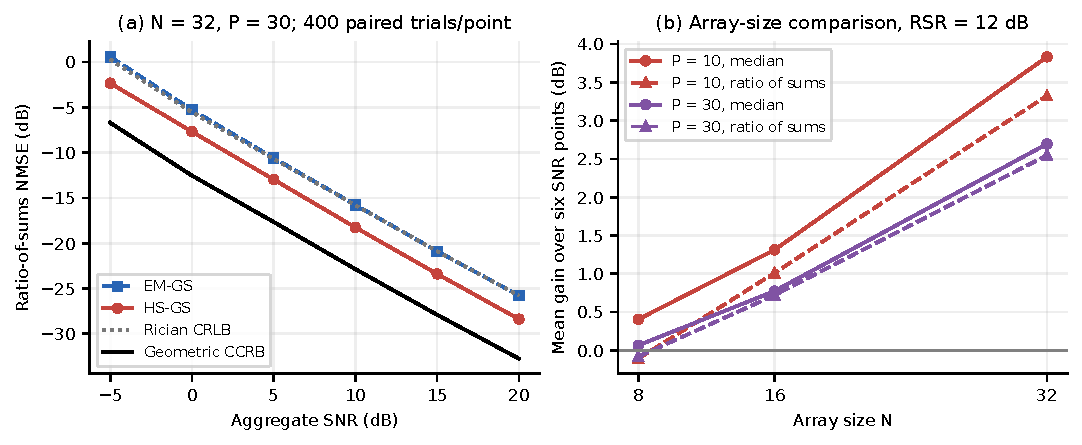
\includegraphics[width=\textwidth]{classical_array.pdf}
\caption{Classical study. Left: NMSE and information references at $N=32$, $P=30$, RSR 12~dB. Right: HS-amplitude gain versus array size for two pilot counts. HS-GS denotes four-sweep HS-amplitude. Solid gain curves average paired medians over six SNRs; dashed curves average ratio-of-sums gains.}
\label{fig:classical}
\end{figure*}
At $N=32$, $P=30$, RSR 12~dB, HS-amplitude gains 2.54--2.97~dB in paired median over EM-GS across six SNRs, averaging 2.70~dB (Fig.~\ref{fig:classical}). Ratio-of-sums gaps are 2.38--2.90~dB. At SNR at least 5~dB, EM-GS is within 0.108~dB of the Rician CRLB. The geometric CCRB is 6.95--7.06~dB below that reference, while HS-amplitude remains 4.37--4.85~dB above it. These local unbiasedness references do not establish efficiency or attainable headroom for the biased filtered estimates.

Averaging two pilot counts and six SNRs, paired-median gains are 0.236, 1.044 and 3.264~dB for $N=8,16,32$. Ratio-of-sums gains are $-0.095$, 0.866 and 2.938~dB. The EM-GS average changes by only 0.120~dB. A larger array supplies more spatial samples of the same path structure; the unrestricted estimator also gains more unknowns. At $N=8$, maximum Hankel rank is four and filtering is bypassed in 42.94\% of trials. A positive median alongside a negative total-error gain shows why aggregation matters.

\subsection{Effective Rank and Filtering Bias}
For the true noiseless Hankel spectrum, define effective rank~\cite{royvetterli2007}
\begin{equation}
 r_{\rm eff}=\exp(-\textstyle\sum_i p_i\log p_i),\qquad \rho=r_{\rm eff}/q.
\end{equation}
A spectrum dominated by a few values has low effective rank even if its algebraic rank is larger. We report median $\rho$ over users and worlds. This true-channel diagnostic is not available to the estimator.
\begin{figure}[!t]
\centering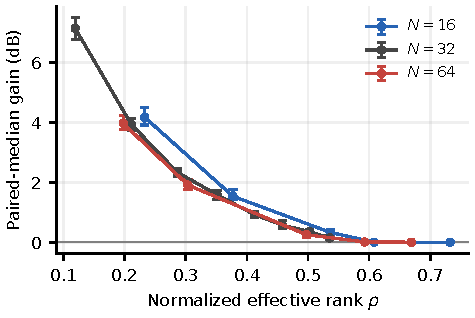
\includegraphics[width=\columnwidth]{effective_rank.pdf}
\caption{Four-sweep HS-amplitude paired-median gain versus true-channel normalized effective rank. Arrays use $P=20$, RSR 10~dB and the same random-SNR distribution. Bars are pointwise paired-bootstrap intervals. This is a diagnostic trend, not an observable switching threshold.}
\label{fig:rank}
\end{figure}
Across the matched array tests, hard-rank benefit generally falls as $\rho$ rises (Fig.~\ref{fig:rank}). At $N=32$, $\rho=0.536$ gives median gain 0.141~dB with interval $[0.090,0.211]$~dB. A value near one-half of capacity marks a small benefit here, not a universal threshold. At $N=16$, $L=14$, $\rho=0.732$, forcing rank seven loses 0.154~dB, with interval $[0.111,0.201]$~dB for the loss.

Adaptive rank does not protect every channel. At $N=32$, $L=14$, SNR 0~dB, HS-amplitude is worse than EM-GS in 47.75\% of 400 worlds. Conversely, selecting below the physical path count is not always harmful: at $L=7$, SNR 0~dB, 78.75\% select below rank seven, while only 8.75\% of all worlds are worse than EM-GS. Removing weak paths can help under noise.

The classical smooth filter gains 0.914, 1.382 and 1.413~dB over four-sweep hard filtering at SNR 0~dB for $L=3,7,14$, respectively. Gains at 10~dB are 0.005, 0.623 and 0.773~dB; the first interval includes zero. Thus improvement over hard truncation does not itself require learning. In the separate fresh sweep study, one hard sweep improves over four in all six cells by 0.275--0.652~dB, with pointwise intervals above zero. More structural processing is not automatically better. Placement comparisons and independently selected one-sweep controls are retained in the supplement.

\subsection{Final Compact Comparison}
\begin{table}[!t]
\caption{Final fresh comparison: 4,032 primary worlds. Lower NMSE is better. Neural scores average three models, not predictions. Time includes initialization and rank-search/refitting where used.}
\label{tab:compact}\centering\footnotesize\setlength{\tabcolsep}{3pt}
\begin{tabular}{@{}lrrrr@{}}\toprule
Method & Weights & NMSE & Time & Severe\\
 & & (dB) & (ms) & (\%)\\\midrule
Learned steps & 10 & $-9.773$ & 1.79 & 22.84\\
Global filtering & 30 & $-11.857$ & 3.41 & 19.56\\
Recurrent adaptation & 148 & $-11.725$ & 4.15 & 19.78\\
Our spectral/state control & 188 & $-13.692$ & 4.87 & 3.10\\
OptShrink, offline & --- & $-13.204$ & 15.81 & 4.46\\
OptShrink, block rank & --- & $-14.144$ & 110.56 & 6.77\\\bottomrule
\end{tabular}
\end{table}
Table~\ref{tab:compact} compares all six methods. Our controller improves on learned steps alone by 3.919~dB, with adjusted interval $[3.789,4.001]$~dB, and on global filtering by 1.835~dB, with interval $[1.805,1.871]$~dB. It improves on the recurrent adaptation by 1.967~dB, with interval $[1.932,2.006]$~dB. It wins 114 of 126 cells against recurrence, with worst observed cell loss 0.176~dB. This is evidence for the tested design under a matched training budget, not a claim that every recurrent controller or published NA-ALISTA is inferior.

Compared with offline-selected OptShrink, our descriptive average gain is 0.488~dB and mean time is about 3.24 times lower. Per-block in-loop rank selection reverses the accuracy ranking: OptShrink gains 0.452~dB, while our measured time is about 22.7 times lower. Our worst primary-cell loss to that selector is 5.848~dB. The comparison includes classical search and all-pilot refitting, but excludes neural training and classical offline tuning. It represents a reusable trained estimator versus additional per-block computation, not a free accuracy gain.

\begin{figure*}[!t]
\centering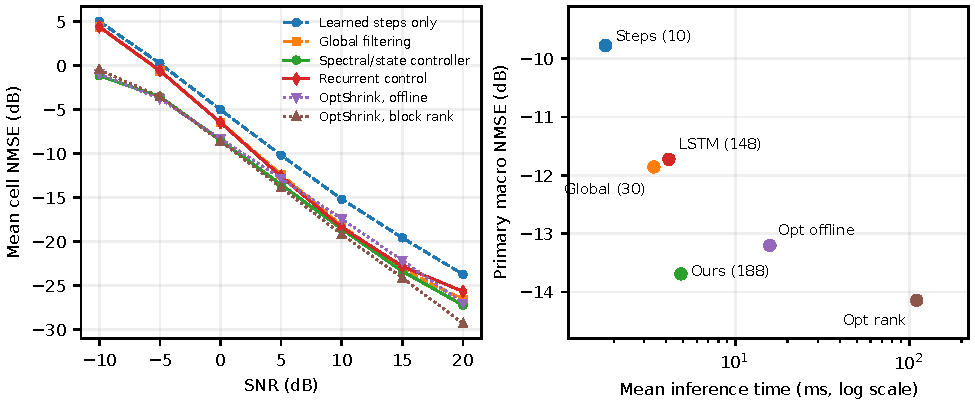
\includegraphics[width=\textwidth]{compact_comparison.pdf}
\caption{Final fresh comparison. Left: each SNR point averages 18 reference/path cells. Right: equal-cell primary accuracy and serial processing time. All methods use the same PyTorch CPU backend. Lines are descriptive averages, not simultaneous per-cell confidence guarantees.}
\label{fig:compact}
\end{figure*}
Figure~\ref{fig:compact} summarizes the SNR and cost trends. The original 188-parameter seed scores are $-13.784$, $-13.449$ and $-13.843$~dB; recurrent scores are $-11.707$, $-11.740$ and $-11.728$~dB. Our two bank averages are $-13.706$ and $-13.682$~dB. These show variation across fitted seeds and fresh observations, not independent training-population replication. The recurrent model is slightly faster and uses fewer parameters. Its observed accuracy gap does not establish its best attainable performance after longer training or a different feature design.

\subsection{Error Aggregation and Earlier Evidence}
Our severe-error rate is 3.10\%, compared with 19.78\% for recurrence, 4.46\% for offline OptShrink and 6.77\% for per-block rank selection. This threshold is not the primary selection objective or a communication-outage metric. At NMSE 0.5, exceedance rates are 19.43\%, 19.12\% and 19.27\% for our estimator and the two OptShrink controls. Lower severe-error frequency does not mean our error distribution dominates theirs.

Pooling linear errors over primary worlds before taking dB gives $-6.664$~dB for ours, $-6.564$~dB for offline OptShrink and $-6.228$~dB for per-block selection. That descriptive measure favors ours over the primary accuracy winner. It gives more influence to large errors, whereas the declared primary score gives every operating cell equal dB weight. We retain the primary rule rather than choosing the aggregation with the most favorable ranking.

Separate earlier studies support the same conditional interpretation. On a narrower RSR 12~dB, 3--7-path population, in-loop OptShrink beats ours by 0.143~dB, with interval $[0.086,0.198]$~dB. A broad offline-tuning study gives ours a 0.537~dB advantage, with adjusted interval $[0.450,0.695]$~dB. A further fresh per-block rank study gives in-loop OptShrink a 0.507~dB advantage, with interval $[0.437,0.562]$~dB. Those banks and protocols remain separate; they are not averaged into the final compact score. The strongest comparator, tuning population and metric must be stated together.

\subsection{Failures and Scope of Robustness}
\begin{table}[!t]
\caption{Separate final stress cells: 32 paired worlds each. NMSE in dB; lower is better. Neither enters selection or the primary average.}
\label{tab:stress}\centering\footnotesize\setlength{\tabcolsep}{4pt}
\begin{tabular}{@{}lrr@{}}\toprule
Method & Weak reference & Nearly noiseless\\
 & SNR 5/RSR 0 dB & SNR 60/RSR 12 dB\\\midrule
Our controller & $-6.842$ & $-6.321$\\
Recurrent adaptation & $-5.623$ & $-20.101$\\
OptShrink, offline & $-10.823$ & $-67.701$\\
OptShrink, block rank & $-12.625$ & $-70.336$\\\bottomrule
\end{tabular}
\end{table}
Weak reference and nearly noiseless observations expose substantial failures (Table~\ref{tab:stress}). At low noise, our filter can erase information that the measurement update already recovers accurately. A separate 32-world diagnostic at SNR 60~dB reaches $-6.647$~dB with the full model, $-44.020$~dB when filtering alone is disabled, and $-65.715$~dB with EM100. Even starting the full learned model at the true channel gives $-6.653$~dB. These post-hoc tests implicate filtering bias; they do not supply a validated switching rule.

Additional checks examine, but do not establish general robustness. Frozen-model tests vary $N\in\{8,16,32,64\}$, $K\in\{2,3,4\}$ and $P\in\{10,20,30\}$ one factor at a time. The gain interval at $N=8$ includes zero. A smaller pilot study reaches $-2.197$~dB at $P=6=2K$ versus $-14.332$~dB at $P=30$, at SNR 5~dB. Regular local identifiability does not ensure useful finite-noise accuracy.

Reference and variance errors also matter. In a separate 32-world SNR 5~dB check, assumed constant reference-phase errors of $\pm10^\circ$ worsen learned NMSE by 2.36--2.47~dB. Phase ramps up to $\pm10^\circ$ lose 0.78--0.84~dB; supplying variance 6~dB too high loses 3.05~dB. A classical position-error simulation reduces structural benefit as element deviations grow. These are simulated mismatch tests, not hardware calibration or unknown-drift solutions.

Input-removal, depth and placement studies are documented separately. More inputs improve average accuracy but not every condition. A reduced-budget 5/10/20-stage comparison finds a 1.977~dB loss for five stages and only 0.181~dB gain for twenty over ten, with nearly doubled time. Corrected learned OptShrink hybrids, simple filter-release rules and a small Transformer pilot fail to establish a better replacement. Their negative results are retained; the Transformer is not a strong matched URformer reproduction.

\section{Discussion and Conclusion}
The classical and learned results share one lesson: structural processing must be judged by the noise it removes, the bias it adds and the work required to choose it. Effective rank explains part of the classical trend, but is a true-channel diagnostic here. A bypass option, learned gate or norm-nonincreasing filter is not per-world protection. Stronger classical tuning changes the ranking and is essential to a credible learned-method claim.

Our estimator is relevant when many received blocks come from a known operating population and can reuse offline training. The final comparison supports improved accuracy over the tested compact controls and offline lookup, while per-block rank-selected OptShrink remains the accuracy winner. Fewer severe errors and lower measured cost are useful but do not establish safety or overall distribution dominance. The network is not necessary for the best primary accuracy, and its advantages do not survive every channel or noise regime.

One present adaptive stage costs $O(NKP+NK^2+K^3+Kmq^2+Kq^3)$. Features still require an SVD and reconstruction a dense solve. Rank selection repeats structural operations across candidates and updates. Parameter count alone is therefore not a computational-cost measure. The measured ratios depend on backend, precision, thread count and block size; larger batches or optimized classical code can change them. Offline training and tuning must also be considered for deployment.

The scope is simulation-based estimation with a calibrated reference and known Gaussian-field-noise variance. Confidence intervals condition on trained models; shared training data and the 20-epoch recurrent budget limit broader inference. No hardware, full-estimator convergence, statistically optimal cubic shrinkage, 2D-array recovery or published-URformer superiority is established. Full LRHD, variational low-rank phase retrieval and other sparse methods remain adapted-comparison gaps, not methods assumed to lose. The 21-input/30-input training/deployment change is disclosed but not causally isolated.

In conclusion, a small self-supervised controller can learn useful spatial filtering without channel labels and avoid per-block search. Paired classical evidence explains why filtering strength, array support and structural bias matter. Fresh matched results establish a conditional accuracy--cost trade-off against strong controls, including an OptShrink variant with better primary accuracy. The observed operating limits are part of the result, not exceptions to a universal superiority claim.

\subsection{Reproducibility}
The supplement gives exact protocols, recurrent equations, numerical rules, earlier results and negative checks. The final audit regenerated all 4,096 worlds, replayed 3,072 representative neural predictions and 64 independent NumPy classical predictions, and independently recalculated headline statistics. Maximum replay difference was $4.40\times10^{-13}$. Seven new tests cover control equivalence, gradients, precision, state isolation, user permutation and deterministic resumption. This is not a replay of every historical experiment. The manuscript archive includes source, figures and compact evidence; full arrays and checkpoints are separate. A permanent public code/data destination remains to be assigned before submission.

\section*{Acknowledgment}
OpenAI's ChatGPT/Codex assisted with manuscript drafting and revision, experiment-code development, and figure-generation scripts. The author is responsible for verifying the content and final submission.
\bibliographystyle{IEEEtran}
\bibliography{references}
\end{document}
